For the main control of the system, a State Machine with singleton pattern design is used. Every state is designed to be as small as possible. For the German Open 2015, we implemented three main states divided on smaller sub-states: move, grasp and deliver (see figure~\ref{fig:SM}).

On the initialization state, the robot receives the map and localizes itself on it. Then we go to state Idle and wait until the tasks are received from the referee box. We divide the complete task into smaller subtask and manage them on the stateNext. 

The first step is always to drive to a specific position with a specific orientation. In this case we would first plan a trajectory on the map, drive to the desired position by following the path waypoints and finally wait there for some seconds. Once the moving task is finished we return to StateNext to check which is the next desired state.

If we want to grasp an object, we would first smoothly approach to the service area and go to stateFindDesiredObject. After localizing the position of the desired object, we grasp it, lay it in our back and return back from the service area. 

In case of delivering an object, we also approach smoothly to the service area but this time we will pick up the object from our back and deliver it on the service area. Finally we return back from the service area and go again to StateNext.

The State Machine framework could be found on GitHub under our Laboratory’s repository: ”autonohm/obviously”.

\begin{figure}[htbp]
	\centering
	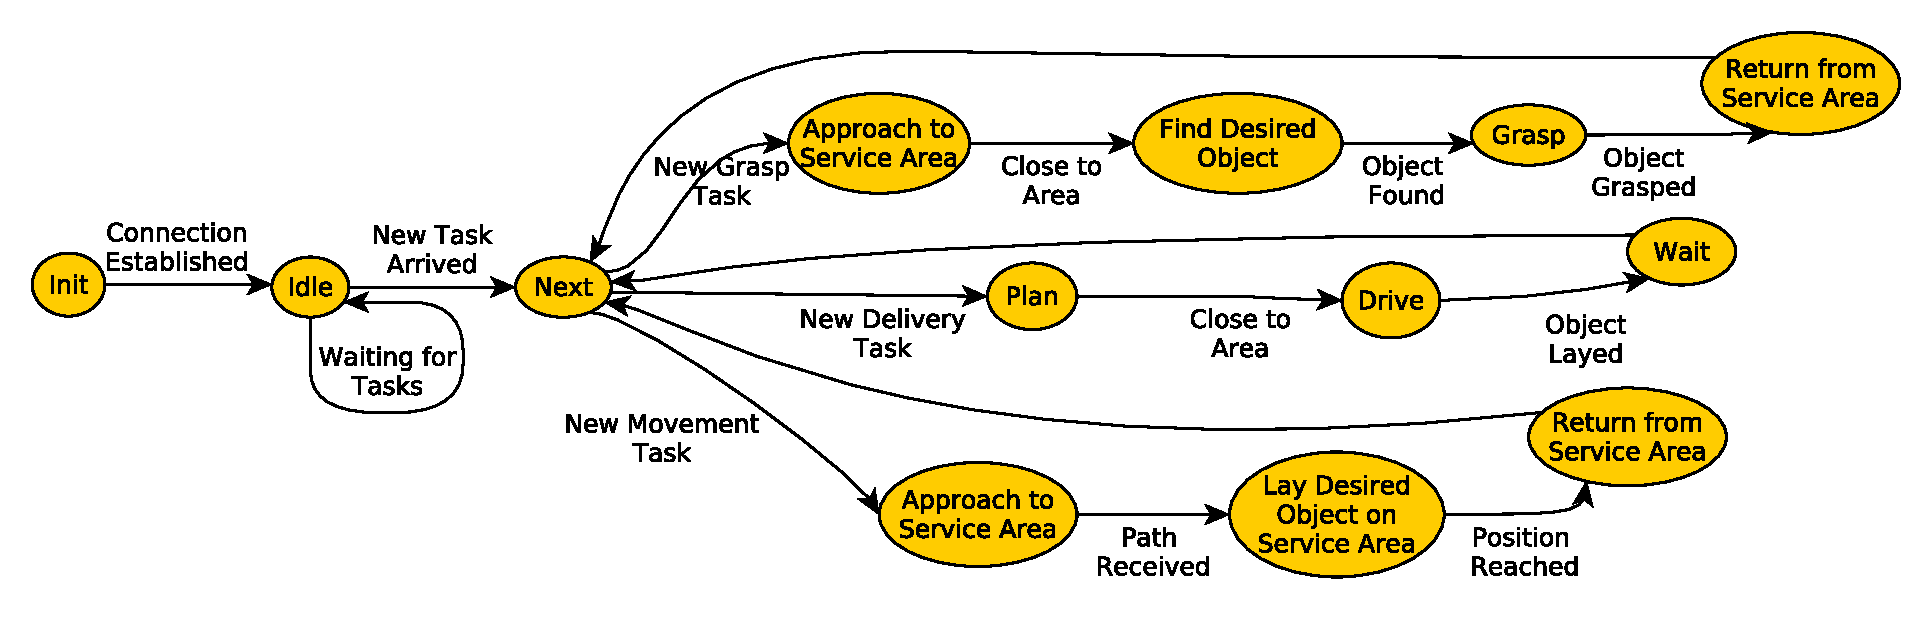
\includegraphics[width=\textwidth]{img/sm}
	\caption{Structure of the Statemachine}
	\label{fig:SM}
\end{figure}